\chapter{Literature study}
\label{chap:rel_work}

We will first examine the effectiveness of existing models on a collection of paintings from 2 different movements.
For this we will need to have a pose estimator, a style transformer and a collection of test data. 

A first method: We will first convert the test data with the style transformer to a painting and then we will apply pose estimation.
The test data will have coordinates of the joints, which we will compare with the results of the pose estimation.
However, the joints are of the original image. How do we convert those coordinates to map to the styled image? 
Problem: This method does not use any real paintings and will be susceptible to the accuracy of the style transformer.  

A second method: We can apply pose estimation to real paintings and then convert them to a realistic image with style transfer.
We can then use pose estimation to the realistic images and compare them with the style transformed results.
This will also require a way to map the results of the real painting to that of the style transformed. 
Problem: While we’re using real paintings now, the results will still depend on the accuracy of style transformer. 

A third method: We can annotate the paintings ourselves and use pose estimation to assess the pose estimation algorithms. 
Problem: We must annotate the paintings ourselves. 

\section{Human Pose estimation}
\label{sec:hpe}

\gls{HPE} aims to detect human features from input data such as images and videos.
It's an elementary part of computer vision with many applications among which are human action recognition (sign language), human tracking (surveillance), and human-computer interaction (video games).
This is an extensively researched area with a diverse range of different techniques.
This chapter will try to give an overview of all the many challenges and proposed solutions.
The focus will be on deep learning models, which have surpassed classical solutions significantly.
Specifically, around 2D monocular \gls{HPE}. \cite{Munea2020}\cite{Zheng2012}\cite{Liu2104}\cite{chen2022}

\subsection{History}
The human body has a high degree-of-freedom due to all the limbs, self-similar parts and body types, which may cause self-occlusion or rare/complex poses.
The variations in configuration are made even larger due to clothing, lighting, foreground occlusion, as well as viewing angles and truncation, among others, as shown in fig. \ref{{fig:hpe_problem_complexity}.
This makes \gls{HPE} one of the most difficult tasks in computer vision. \cite{jain2014}\cite{Chen2000}

\subsubsection{Early models}

\subsection{Representation}

There are several ways that the pose can be represented.
Depending on the needs of the problem you can have a skeleton-base, contour-base, or volume-base solution. \ref{fig:pose_representation} \cite{Chen2000}

Skeleton-based model:
The skeleton is build of a tree-structured set of key-points that represent the joints of the human body.
These can be explicitly described by their coordinates in 2D or 3D space.
More suitable for a \gls{CNN} is a heatmap which constructs a 2D Gaussian kernel around the key-point. \cite{SWARH}

The skeleton-based model "is limited in representing texture and shape information." \cite{Zheng2012}

Contour representation:


Volume representation:
Volume representation is a 3D mesh that represents the human body.


Volume representation creates a complete mesh which is too much information for what we’re working with.​
The keypoints representation is exactly what we need.

We only need to be aware of the most essential joints to label a pose.


There are several ways that the human body joints/keypoints are represented.
A first distinction is 2D and 3D

Top-Down
Regression-based, Heatmap-based, video-based, model compression-based.

Bottom-Up
One stage, two-stage

Pose estimation can be achieved in a number of different ways.
There are popular 2 methods: top-down \cite{alphapose} and bottom-up \cite{blazepose}\cite{openpose}.
The algorithms are further categorized in single-person \cite{blazepose} and multi-person \cite{alphapose}\cite{openpose}\cite{fcpose}

\begin{figure}
	\centering
	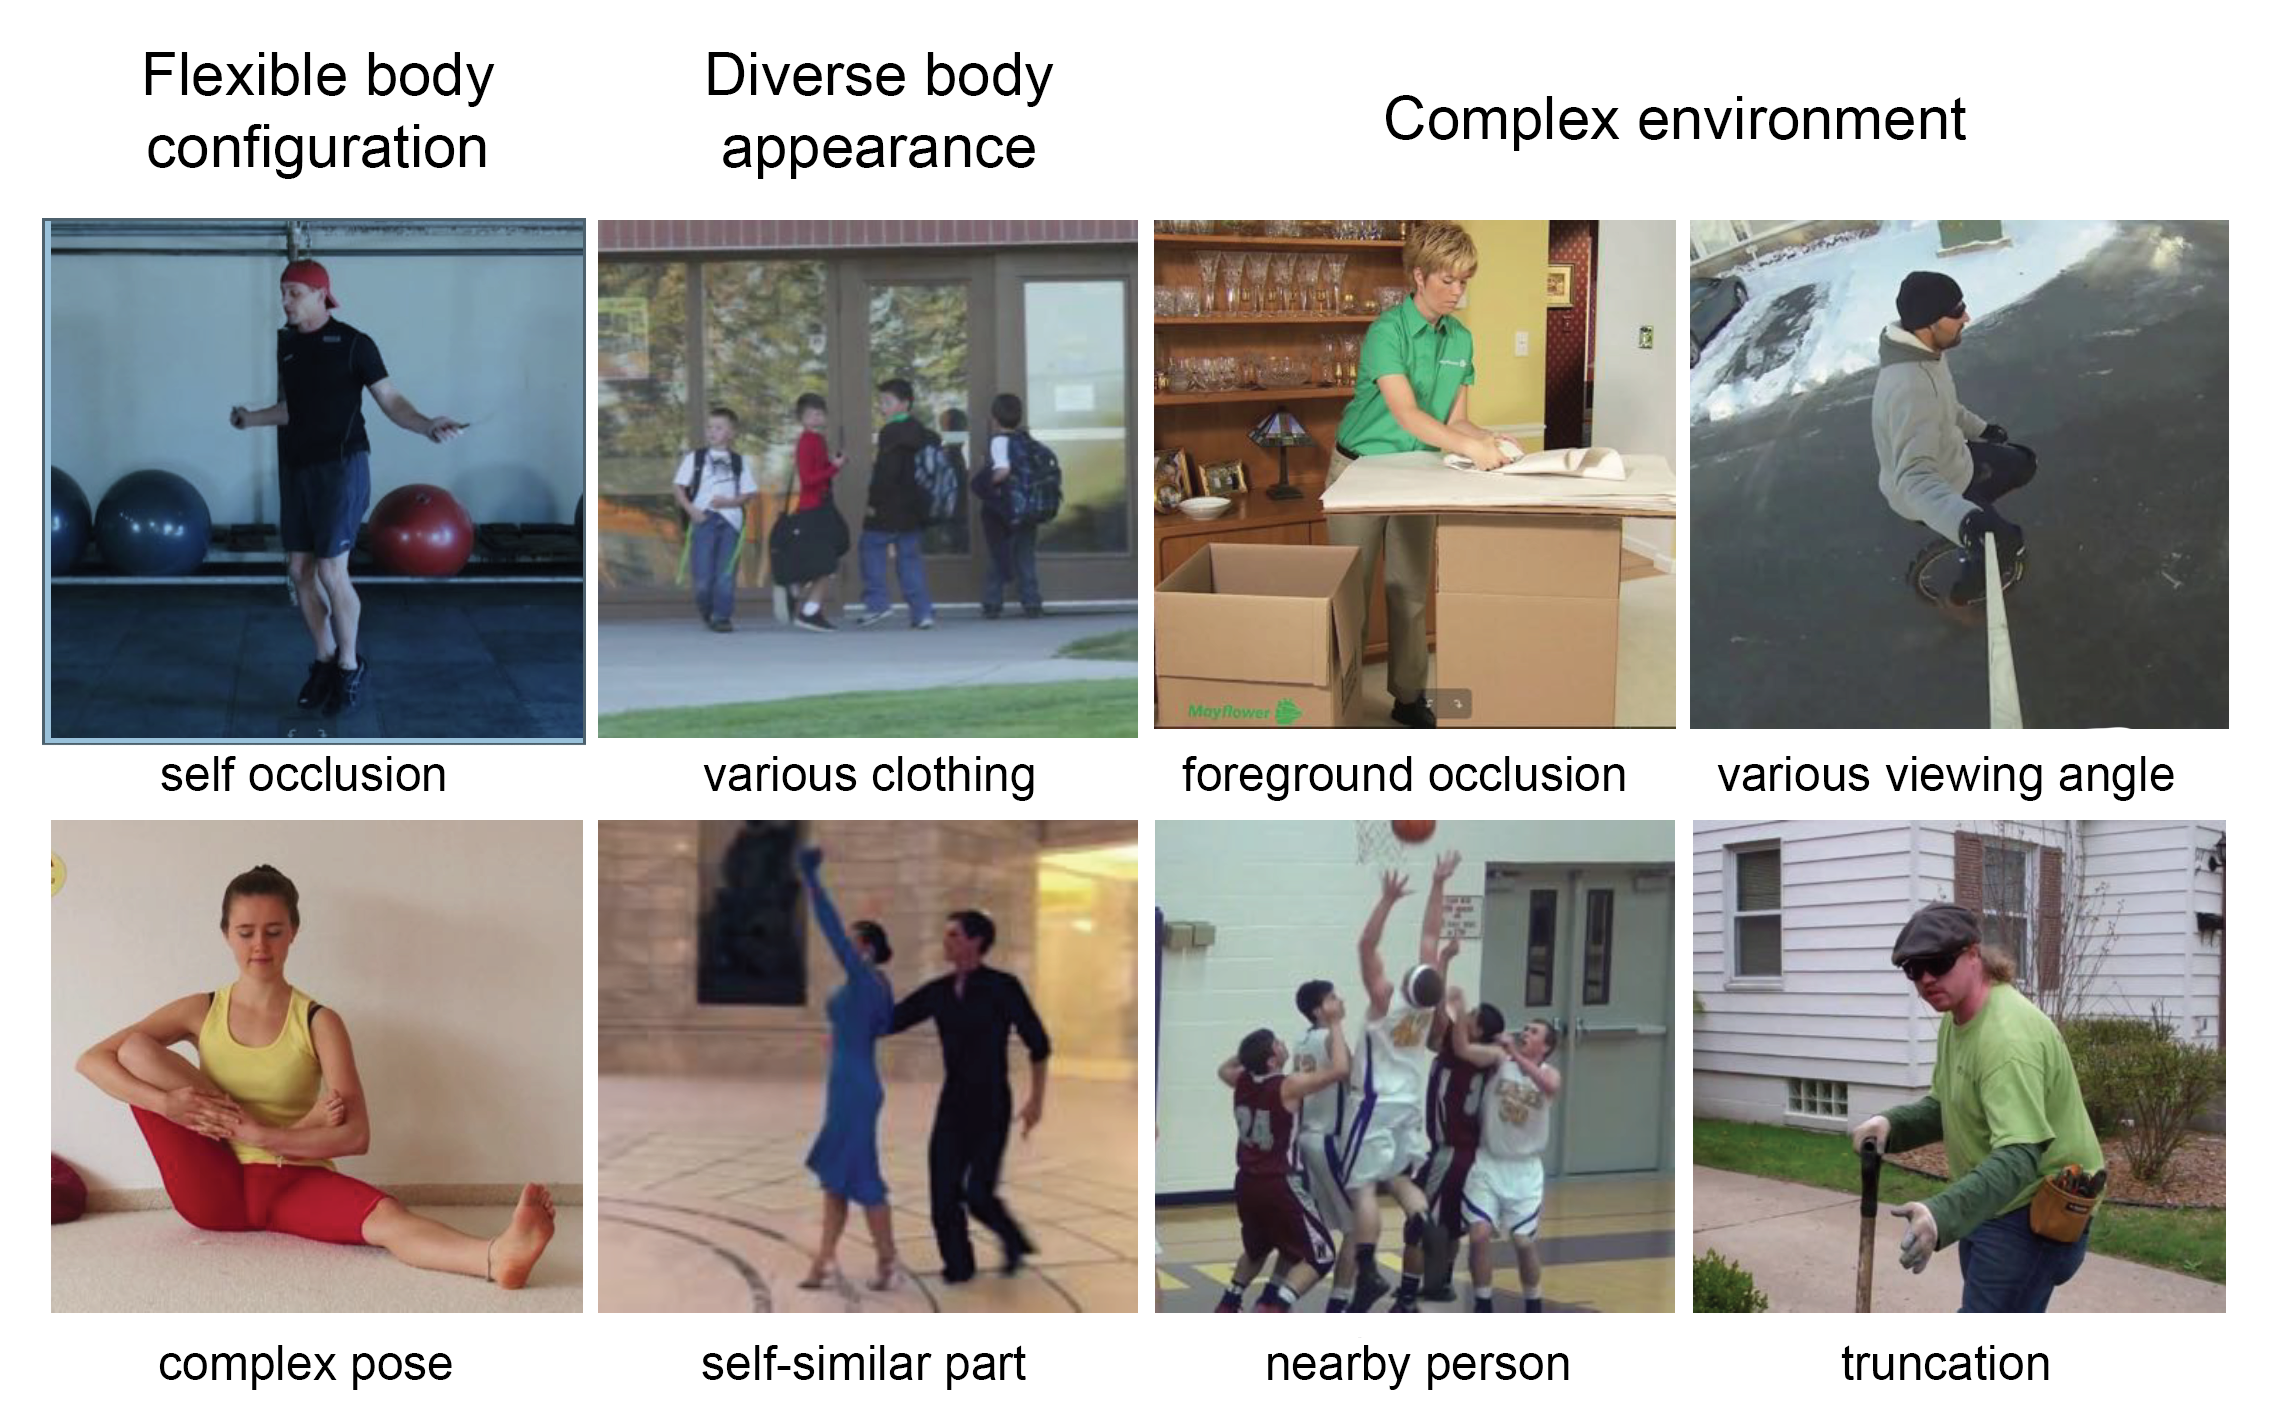
\includegraphics[width=1\textwidth]{hpe_problem_complexity}
	\caption{The various challenges HPE solutions face. Images from \gls{MPII} dataset. \cite{Andriluka2014}\cite{Chen2000}}
	\label{fig:hpe_problem_complexity}
\end{figure}

\begin{figure}
	\centering
	\subcaptionbox{Skeleton \label{fig:pose_representation_skeleton}}{%
		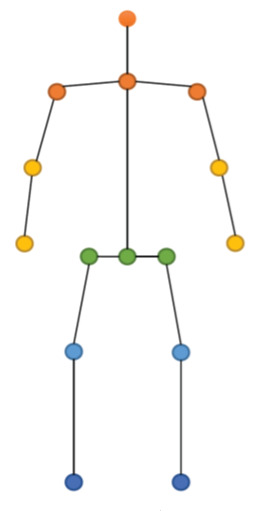
\includegraphics[width=0.3\textwidth]{pose_representation_skeleton}%
	}
	\subcaptionbox{Contour \label{fig:pose_representation_contour}}{%
		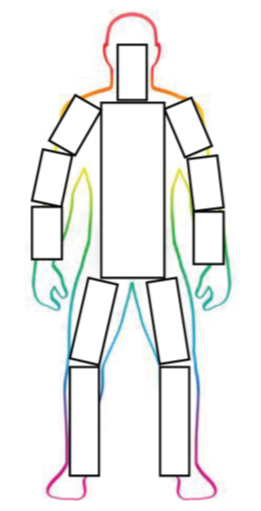
\includegraphics[width=0.3\textwidth]{pose_representation_contour}%
	}
	\subcaptionbox{Volume \label{fig:pose_representation_volume}}{%
		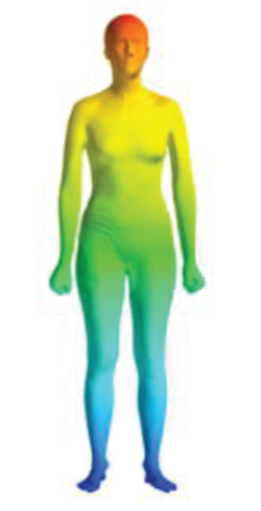
\includegraphics[width=0.3\textwidth]{pose_representation_volume}%
	}
	\caption{Models for pose representation \cite{Zheng2012}}
	\label{fig:pose_representation}
\end{figure}

\subsection{Top-down}

\section{Image Style Transfer}
\label{sec:ist}